\documentclass[11pt, a4paper, twoside]{article}   	% use "amsart" instead of "article" for AMSLaTeX format

\usepackage{geometry}                		% See geometry.pdf to learn the layout options. There are lots.
\usepackage{pdfpages}
\usepackage{caption}
\usepackage{minted}
\usepackage[german]{babel}			% this end the next are needed for german umlaute
\usepackage[utf8]{inputenc}
\usepackage{color}
\usepackage{graphicx}
\usepackage{titlesec}
\usepackage{fancyhdr}
\usepackage{lastpage}
\usepackage{hyperref}
% http://www.artofproblemsolving.com/wiki/index.php/LaTeX:Symbols#Operators
% =============================================
% Layout & Colors
% =============================================
\geometry{
   a4paper,
   total={210mm,297mm},
   left=20mm,
   right=20mm,
   top=20mm,
   bottom=30mm
 }	

\definecolor{myred}{rgb}{0.8,0,0}
\definecolor{mygreen}{rgb}{0,0.6,0}
\definecolor{mygray}{rgb}{0.5,0.5,0.5}
\definecolor{mymauve}{rgb}{0.58,0,0.82}

\setcounter{secnumdepth}{4}


% the default java directory structure and the main packages
\newcommand{\srcDir}{../src/main/java}
\newcommand{\srcTestDir}{../src/test/java}
\newcommand{\resourcesTestDir}{../src/test/resources}
\newcommand{\mainPackageDir}{\srcDir/at/fh/ooe/swe4/fx/campina}
\newcommand{\viewDir}{\mainPackageDir/view}
\newcommand{\viewApiDir}{\viewDir/api}
\newcommand{\viewBuilderDir}{\mainPackageDir/component/builder}
\newcommand{\viewAnnotationDir}{\mainPackageDir/view/annotation}
\newcommand{\viewLoginDir}{\viewDir/admin/login}
\newcommand{\viewUserDir}{\viewDir/admin/user}
\newcommand{\viewMenuDir}{\viewDir/admin/menu}
\newcommand{\viewOrderDir}{\viewDir/admin/order}
\newcommand{\jpaDir}{\mainPackageDir/jpa}
\newcommand{\imagesDir}{images}
% the default subsection headers
\newcommand{\ideaSection}{Lösungsidee}
\newcommand{\sourceSection}{Source-Code}
\newcommand{\testSection}{Tests}

% =============================================
% Code Settings
% =============================================
\newenvironment{code}{\captionsetup{type=listing}}{}
\newmintedfile[javaSourceFile]{java}{
	linenos=true, 
	frame=single, 
	breaklines=true, 
	tabsize=2,
	numbersep=5pt,
	xleftmargin=10pt,
	baselinestretch=1,
	fontsize=\footnotesize
}
\newmintinline[inlineJava]{java}{}
\newminted[javaSource]{java}{
	breaklines=true, 
	tabsize=2,
	autogobble=true,
	breakautoindent=false
}
\newmintedfile[xmlSourceFile]{xml}{
	linenos=true, 
	frame=single, 
	breaklines=true, 
	tabsize=2,
	numbersep=5pt,
	xleftmargin=10pt,
	baselinestretch=1,
	fontsize=\footnotesize
}
\newmintedfile[propertiesFile]{properties}{
	linenos=true, 
	frame=single, 
	breaklines=true, 
	tabsize=2,
	numbersep=5pt,
	xleftmargin=10pt,
	baselinestretch=1,
	fontsize=\footnotesize
}
% =============================================
% Page Style, Footers & Headers, Title
% =============================================
\title{Übung 3}
\author{Thomas Herzog}

\lhead{Übung 3}
\chead{}
\rhead{
\includegraphics[scale=0.10]{FHO_Logo_Students.jpg}}

\lfoot{S1310307011}
\cfoot{}
\rfoot{ \thepage / \pageref{LastPage} }
\renewcommand{\footrulewidth}{0.4pt}
% =============================================
% D O C U M E N T     C O N T E N T
% =============================================
\pagestyle{fancy}
\begin{document}
\setlength{\headheight}{15mm}
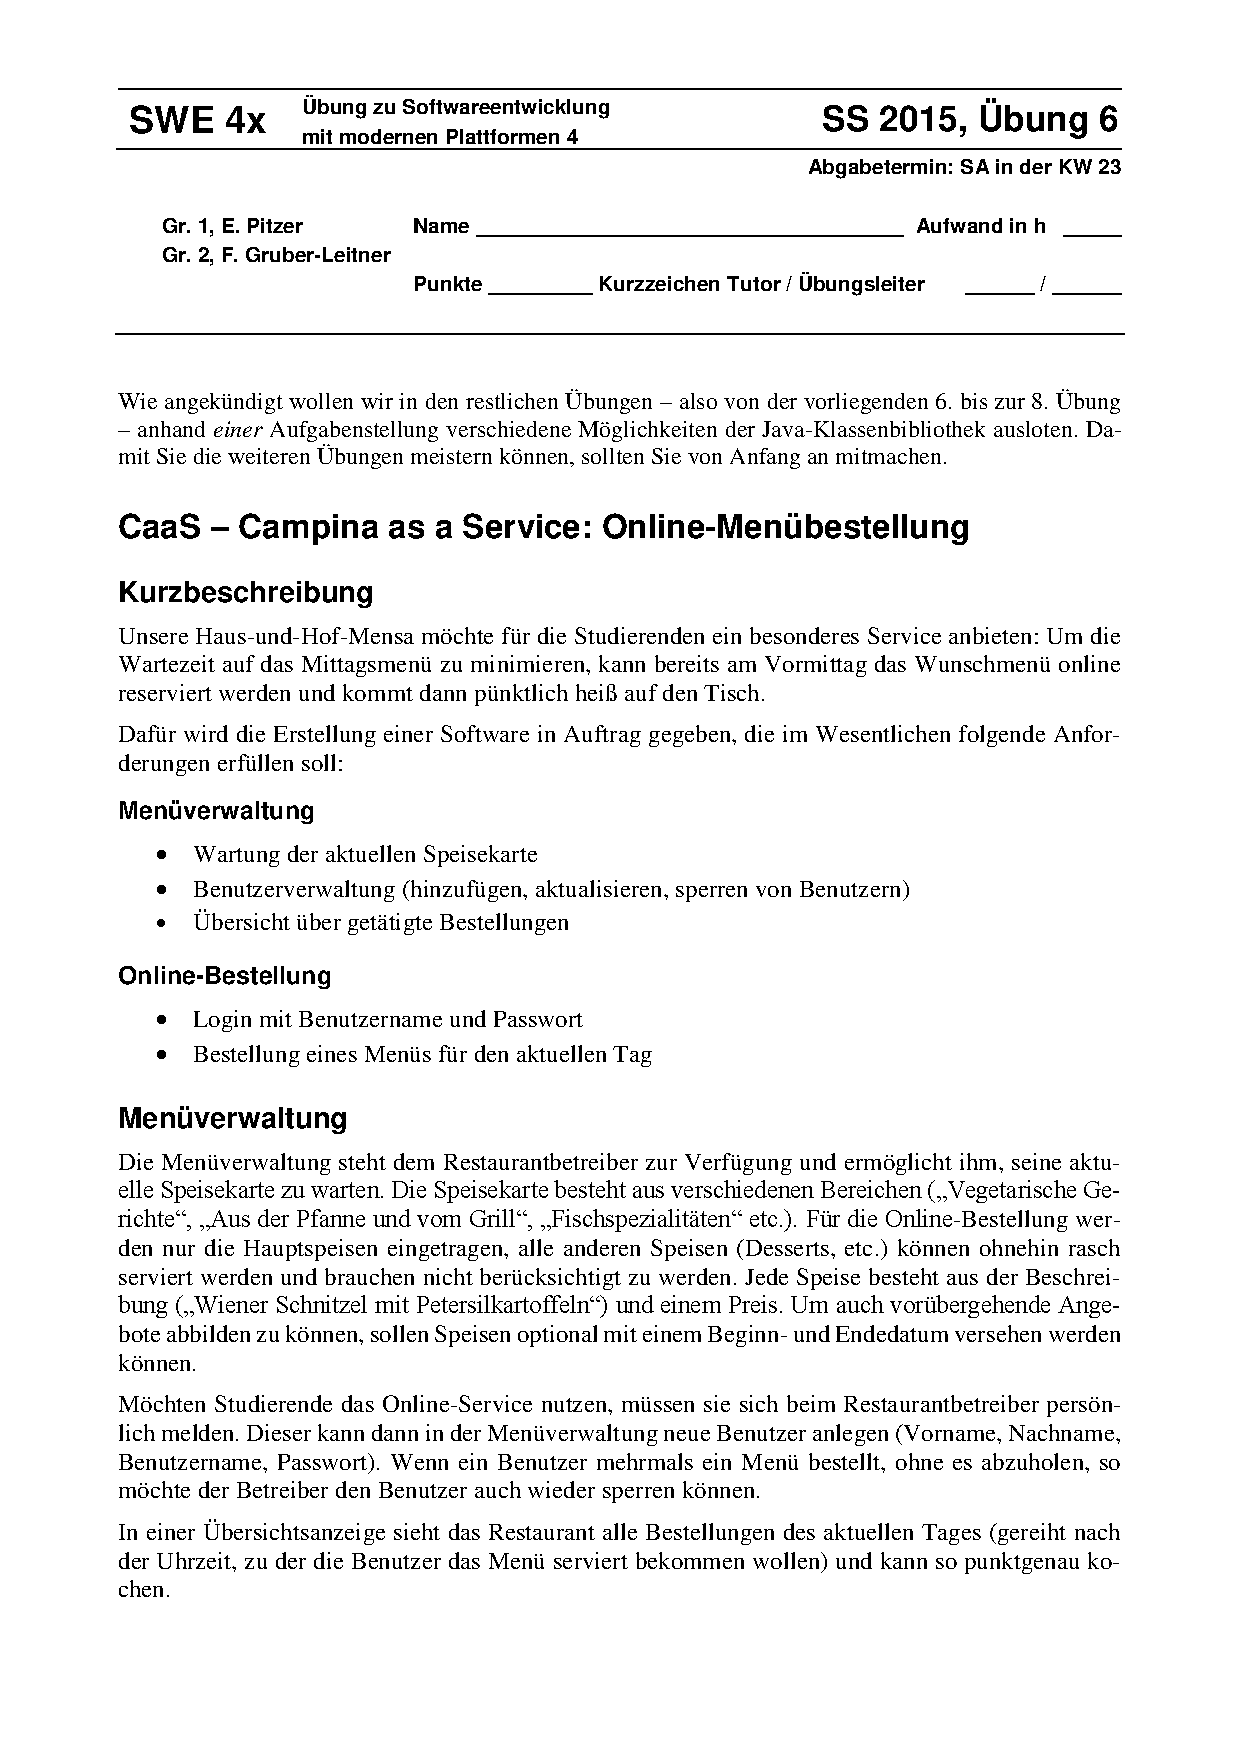
\includepdf[pages={1-2}]{Swe4xA06-BB.pdf}
{\color{myred}
	\section
		{Campina as a Service}
}

\subsection{\ideaSection}
Folgend ist die Dokumentation für die Aufgabenstellung Campina as a Service angeführt. \\
Bei dieser Aufgabenstellung soll in Bezug auf die Softwarearchitektur wie folgt vorgegangen werden.\\\\
\begin{enumerate}
	\item Das Datenmodell soll über POJOs abgebildet werden, die nicht direkt verwendet werden.
	\item Der Zugriff auf die Datenkomponenten einer Entität innerhalb der Views soll über eigene Models abgebildet werden.
	\item Die einzelnen View Teile sollen über eigenen Klassen abgebildet werden, die die View aufbauen un die View Logic beinhalten.
	\item Eigenen Kontroller Implementierungen reagieren auf die ActionEvents der Buttons, die Operationen auf den Entitäten anwenden.
	\item In der nächsten Stufe sollen die Datenzugriffe über DAOs abgebildet werden, die in den Kontroller Implementierungen verwendet werden.
\end{enumerate}
Folgende Abbildung zeigt den prinzipiellen Aufbau aller Formulare.\\
Da die Entitäten nur wenige Skalare Datenkomponenten enthalten, abgesehen von den 1-n, ... Beziehungen, soll hier eine einfache Form angewendet werden.\\
Diese Views können in Zukunft auch noch abgeändert und die List Daten anders dargestellt werden. 
\begin{figure}[H]
	\centering
	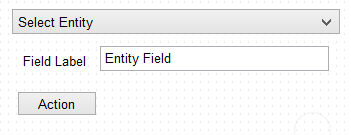
\includegraphics[scale=1]{\imagesDir/mock_form.PNG}
	\caption
	{Formularaufbau}
\end{figure}
Um den folgenden Aufwand der Formulare zu verringern und die Konsistenz der Fromulare zu erhalten, soll eine Komponente entworfen werden, die in der Lage ist deklarativeKlassen oder Methoden Annotationen bzw. deren enthaltenen Informationen zu verarbeiten und ein Formular zu generieren.\\\\
Um zu Vermeiden das wahrlos Referenzen durch die Klassen gezogen werden, soll eine Kontext implementiert werden, der in der Lage ist die Nötigen Informationen und Referenzen zu verwalten, damit sie in den Implementierungen verwendet werden können.\\\\
Die Implementierungen werden in Javadoc und in der folgenden Dokumentation beschrieben.

\newpage
\subsection{\sourceSection (Implementation View API)}
Folgend ist der Source der View API Implementierungen der Übung angeführt.\\

\subsubsection{AbstractViewModel.java}
Folgende abstrakte Klasse stellt die root Klasse für alle View Models dar, die eine Entität verwalten.
\begin{code}
	\caption{AbstractViewModel.java}
	\javaSourceFile{\viewApiDir/AbstractViewModel.java}
\end{code}

\subsubsection{IdHolder.java}
Folgendes Interface markiert eine Klasse oder ein anderes Interface als IdHolder.
\begin{code}
	\caption{IdHolder.java}
	\javaSourceFile{\viewApiDir/IdHolder.java}
\end{code}
\newpage

\subsubsection{ViewHandler.java}
Folgendes Interface spezifiziert einen View Handler, der einen Teilbaum einer Scene verwaltet.
\begin{code}
	\caption{ViewHandler.java}
	\javaSourceFile{\viewApiDir/ViewHandler.java}
\end{code}
\newpage

\subsubsection{EventHandlerFactory.java}
Folgendes Interface spezifiziert eine Event Hadnler Factory die Events registriert und die registrierten Events in Form einer Map liefert.
\begin{code}
	\caption{EventHandlerFactory.java}
	\javaSourceFile{\viewApiDir/EventHandlerFactory.java}
\end{code}
\newpage


\newpage
\subsection{\sourceSection (Implementation View Annotation)}
Folgend ist der Source der Annotation der Übung angeführt.\\

\subsubsection{FormField.java}
Folgende Annotation markiert eine Methode als ein Form Field.\\
Diese Annotation wird dazu verwendet und die Form zu erstellen und zu verwalten.
\begin{code}
	\caption{FormField.java}
	\javaSourceFile{\viewAnnotationDir/FormField.java}
\end{code}
\newpage

\subsubsection{SelectFormField.java}
Folgende Annotation markiert eine Methode als einen Data Provider für ein Formularfeld vom Type Select.
\begin{code}
	\caption{SelectFormField.java}
	\javaSourceFile{\viewAnnotationDir/SelectFormField.java}
\end{code}
\newpage

\subsubsection{EventHandlerFactories.java}
Folgende Annotation kann in der Formfield Annotation verwendet werden um EventHandlerFactories für diese Formularfeld zu definieren.
\begin{code}
	\caption{EventHandlerFactories.java}
	\javaSourceFile{\viewAnnotationDir/EventHandlerFactories.java}
\end{code}
\newpage

\newpage
\subsection{\sourceSection (Implementation View Component Buidler)}
Folgend ist der Source der Komponenten Builder von JavaFX Komponenten der Übung angeführt.\\
Dieser Ansatz ist in Zukunft in Frage zu stellen, ob sich lohnt das erstellen der Komponenten auszulagern.\\

\subsubsection{AbstractFxComponentBuilder.java}
Folgende abstrakte Klasse stellt den root aller Builder Implementierungen dar und zwing die abgeleiteten Klassen für einen konkreten Typ der Builder zu sein.
\begin{code}
	\caption{AbstractFxComponentBuilder.java}
	\javaSourceFile{\viewBuilderDir/api/AbstractFxComponentBuilder.java}
\end{code}

\subsubsection{DuplicateKeyException.java}
Folgende Klasse stellt die Exceptiond ar um anzuzeigen ob sich doppelte Ids in der Scene befinden. Wird aber nur im Buidler verwendet, da es mir schwer viel alle Ids in allen Handlern zu überprüfen um sicherzustellen dass keine Duplikate bezüglich den Ids auftreten.
\begin{code}
	\caption{DuplicateKeyException.java}
	\javaSourceFile{\viewBuilderDir/exception/DuplicateKeyException.java}
\end{code}

\newpage
\subsubsection{MenuBarBuilder.java}
Folgende Klasse stellt den Builder für MenuBar dar.
\begin{code}
	\caption{MenuBarBuidler.java}
	\javaSourceFile{\viewBuilderDir/impl/MenuBarBuilder.java}
\end{code}
\newpage

\newpage
\subsubsection{MenuBuilder.java}
Folgende Klasse stellt den Builder für Menu dar.
\begin{code}
	\caption{MenuBuidler.java}
	\javaSourceFile{\viewBuilderDir/impl/MenuBuilder.java}
\end{code}
\newpage

\subsubsection{MenuItemBuilder.java}
Folgende Klasse stellt den Builder für MenuItem dar.
\begin{code}
	\caption{MenuItemBuidler.java}
	\javaSourceFile{\viewBuilderDir/impl/MenuItemBuilder.java}
\end{code}
\newpage


\newpage
\subsection{\sourceSection (Implementation Form Handler)}
Folgend ist der Source des Form Handling angeführt.\\

\subsubsection{FormUtils.java}
Folgende Klasse stellt Utilities für das Form Handling zur Verfügung.
\begin{code}
	\caption{FormUtils.java}
	\javaSourceFile{\viewDir/form/FormUtils.java}
\end{code}
\newpage

\subsubsection{FormHandler.java}
Dieser Handler erstellt das Formular und verwaltet dieses Formular.
\begin{code}
	\caption{FormHandler.java}
	\javaSourceFile{\viewDir/form/FormHandler.java}
\end{code}
\newpage

\newpage
\subsection{\sourceSection (Implementation Data Model)}
Folgend ist der Source der Daten Modelle angeführt.\\
Dieses Model kann dann in weiterer Folge zu JPA Entitäten umgewandelt werden.

\subsubsection{AbstractEntity.java}
Folgende abstrakte Klasse stellt die root Entität für alle Entitäten dar und implementiert bereits \inlineJava{_getId(); setId();}, wobei \inlineJava{_getId()} dafür getdacht ist um die private Datenkomponente id zu erhalten sondern um die Subklassen dazu zu zwingen, dass sie \inlineJava{getId()} überschreiben und ein \inlineJava{@Id} Mapping definieren. (JPA relevant)

\begin{code}
	\caption{AbstractEntity.java}
	\javaSourceFile{\jpaDir/api/AbstractEntity.java}
\end{code}
\newpage

\subsubsection{Day.java}
Folgende Enumeration spezifiziert die zuer Verfügung stehenden Tage und auch einen Label, der in einen Produktivsystem über Keys in Form von String, Enumeration abgebildet werden sollte um Internationalisierung zu realisieren.\\
Dieser Datentyp kann in JPA mit Hibernate nativ gemapped werden ansonsten müsste man die Enumeration in einen String \inlineJava{enum.name()} serialisieren und wieder zu einer Emuneration de-serialisieren,w as sich aber als nicht schwierig herausstellen sollte.
\begin{code}
	\caption{Day.java}
	\javaSourceFile{\jpaDir/constants/Day.java}
\end{code}
\newpage

\subsubsection{User.java}
Folgende Klasse stellt den User auf der Datenbank dar.
\begin{code}
	\caption{User.java}
	\javaSourceFile{\jpaDir/User.java}
\end{code}
\newpage

\subsubsection{Menu.java}
Folgende Klasse stellt den Menu auf der Datenbank dar.
\begin{code}
	\caption{Menu.java}
	\javaSourceFile{\jpaDir/Menu.java}
\end{code}
\newpage

\subsubsection{MenuEntry.java}
Folgende Klasse stellt den Menu Eintrag auf der Datenbank dar.\\
Ein Menu (Fischtag) kann mehrere Gerichte haben (Forelle, Zander, ...)
\begin{code}
	\caption{MenuEntry.java}
	\javaSourceFile{\jpaDir/MenuEntry.java}
\end{code}
\newpage

\subsubsection{Order.java}
Folgende Klasse stellt den Order Eintrag auf der Datenbank dar.\\
Ein Menu (Fischtag) kann mehrere Gerichte haben (Forelle, Zander, ...)
\begin{code}
	\caption{Order.java}
	\javaSourceFile{\jpaDir/Order.java}
\end{code}
\newpage

\subsubsection{LoginEvent.java}
Folgende Klasse stellt den Login Eintrag auf der Datenbank dar.\\
Ermöglicht die Nachverfolgbarkeit der Logins der Benutzer.
\begin{code}
	\caption{LoginEvent.java}
	\javaSourceFile{\jpaDir/LoginEvent.java}
\end{code}
\newpage

\subsubsection{EntityCache.java}
Folgende Klasse dient zu Simulation einer Datenbank damit Daten innerhalb der Laufzeit persistent gehalten werden.

\begin{code}
	\caption{EntityCache.java}
	\javaSourceFile{\jpaDir/EntityCache.java}
\end{code}
\newpage

\newpage
\subsection{\sourceSection (Implementation Login View)}
Folgend ist der Source der Login View angeführt.

\subsubsection{LoginModel.java}
Folgend ist das Login Model angeführt welches für das Login Formular verwendet wird.
\begin{code}
	\caption{LoginModel.java}
	\javaSourceFile{\viewLoginDir/model/LoginModel.java}
\end{code}
\newpage

\subsubsection{LoginEventControl.java}
Folgend ist die Klasse angeführt, welche die Actions behandelt, wie Speichern, Löschen, usw.
\begin{code}
	\caption{LoginEventControl.java}
	\javaSourceFile{\viewLoginDir/control/LoginEventControl.java}
\end{code}
\newpage

\subsubsection{LoginTabViewHandler.java}
Folgend ist der ViewHanddler der LoginTab angeführt. Sie stellt einen View Teil der Scene dar und implementiert \inlineJava{ViewHandler<T>} Interface.
\begin{code}
	\caption{LoginTabViewHandler.java}
	\javaSourceFile{\viewLoginDir/part/LoginTabViewHandler.java}
\end{code}
\newpage


\newpage
\subsection{\sourceSection (Implementation User View)}
Folgend ist der Source der User View angeführt.

\subsubsection{UserModel.java}
Folgend ist das User Model angeführt welches für das User Formular verwendet wird.
\begin{code}
	\caption{UserModel.java}
	\javaSourceFile{\viewUserDir/model/UserModel.java}
\end{code}
\newpage

\subsubsection{UserEventControl.java}
Folgend ist die Klasse angeführt, welche die Actions behandelt, wie Speichern, Löschen, usw.
\begin{code}
	\caption{UserEventControl.java}
	\javaSourceFile{\viewUserDir/control/UserEventControl.java}
\end{code}
\newpage

\subsubsection{UserTabViewHandler.java}
Folgend ist der ViewHanddler der UserTab angeführt. Sie stellt einen View Teil der Scene dar und implementiert \inlineJava{ViewHandler<T>} Interface.
\begin{code}
	\caption{UserTabViewHandler.java}
	\javaSourceFile{\viewUserDir/part/UserTabViewHandler.java}
\end{code}
\newpage

\newpage
\subsection{\sourceSection (Implementation Menu View)}
Folgend ist der Source der Menu View angeführt.

\subsubsection{MenuModel.java}
Folgend ist das Menu Model angeführt welches für das Menu Formular verwendet wird.
\begin{code}
	\caption{MenuModel.java}
	\javaSourceFile{\viewMenuDir/model/MenuModel.java}
\end{code}
\newpage

\subsubsection{MenuEventControl.java}
Folgend ist die Klasse angeführt, welche die Actions behandelt, wie Speichern, Löschen, usw.
\begin{code}
	\caption{MenuEventControl.java}
	\javaSourceFile{\viewMenuDir/control/MenuEventControl.java}
\end{code}
\newpage

\subsubsection{MenuEntryModel.java}
Folgend ist das Menu-Eintrag Model angeführt welches für das Menu-Eintrag Formular verwendet wird.
\begin{code}
	\caption{MenuEntryModel.java}
	\javaSourceFile{\viewMenuDir/model/MenuEntryModel.java}
\end{code}
\newpage

\subsubsection{MenuEntryEventControl.java}
Folgend ist die Klasse angeführt, welche die Actions behandelt, wie Speichern, Löschen, usw.
\begin{code}
	\caption{MenuEntryEventControl.java}
	\javaSourceFile{\viewMenuDir/control/MenuEntryEventControl.java}
\end{code}
\newpage

\subsubsection{MenuTabViewHandler.java}
Folgend ist der ViewHanddler der MenuTab angeführt. Sie stellt einen View Teil der Scene dar und implementiert \inlineJava{ViewHandler<T>} Interface.
\begin{code}
	\caption{MenuTabViewHandler.java}
	\javaSourceFile{\viewMenuDir/part/MenuTabViewHandler.java}
\end{code}
\newpage



\newpage
\subsection{\sourceSection (Implementation Order View)}
Folgend ist der Source der Order View angeführt.

\subsubsection{OrderModel.java}
Folgende Klasse representiert das View Model für Order Entitäten.

\begin{code}
	\caption{OrderModel.java}
	\javaSourceFile{\viewOrderDir/model/OrderModel.java}
\end{code}
\newpage

\subsubsection{OrderEventHandler.java}
Folgend ist die Klasse angeführt, welche die Actions behandelt, wie Speichern, Löschen, usw.

\begin{code}
	\caption{OrderEventHandler.java}
	\javaSourceFile{\viewOrderDir/control/OrderEventHandler.java}
\end{code}
\newpage

\newpage
\subsection{\sourceSection (Implementation Main Scene)}
Folgend ist der Source der Main Scene angeführt.

\subsubsection{MainSceneViewHandler.java}
Diese Klasse baut sich die Scene auf initialisiert sie. In Zukunft könnte sie auch das wechseln zwischen View Teilen verwalten (Tab Visibility, usw.).\\
Dies könnte über Menu-Einträge erfolgen, die hier erstellt und verwaltet werden.

\begin{code}
	\caption{MainSceneViewHandler.java}
	\javaSourceFile{\viewDir/scene/MainSceneViewHandler.java}
\end{code}
\newpage

\subsubsection{MainSceneEventHandlerFactory.java}
Folgend ist der Source der EVentHandlerFactory für die Main Scene angeführt, diedie Events für die Window Menus erstellt.
\begin{code}
	\caption{MainSceneEventHandlerFactory.java}
	\javaSourceFile{\viewDir/scene/MainSceneEventHandlerFactory.java}
\end{code}
\end{document}  